\chapter{ความรู้เบื้องต้นเกี่ยวกับ Python}

\section{Python คืออะไร}

ในปี ค.ศ. 1980 Mr. Guido van Rossum ได้พัฒนาภาษาโปรแกรมมิ่งขึ้นมาและให้ชื่อว่าภาษา Python และเผยแพร่ให้ใช้งานสู่สาธารณชนในปี ค.ศ. 1991 \cite{Gui19} Python เป็นภาษาโปรแกรมคอมพิวเตอร์ระดับสูงซึ่งไวยากรณ์ของภาษาระดับสูงนี้จะใกล้เคียงคำในภาษาอังกฤษทั่วไป \cite{All15}  Python ถูกใช้ในการสร้างโมบายแอพพลิเคชั่น เว็บไซต์ เว็บแอพพลิเคชั่น ออนไลน์เซอร์วิส รวมทั้งใช้ใน การวิเคราะห์ข้อมูลและคำนวณ ทางคณิตศาสตร์และวิทยาศาสตร์อย่างแพร่หลาย  ตัวอย่าง ออนไลน์เซอร์วิสที่พัฒนาขึ้นด้วยภาษา Python ได้แก่ Instagram, Uber, Pinterest, Reddit, Spotify และ Dropbox \cite{Shu19} โดยในระยะหลายปี ที่ผ่านมานี้ Python ได้รับความนิยมสูงขึ้นเรื่อยๆ โดยในเดือนมิถุนายน 2562 ดัชนีความนิยมภาษาโปรแกรมมิ่ง TIOBE ได้แสดงให้เห็นว่า Python เป็นภาษาโปรแกรมมิ่ง ที่ได้รับความนิยมเป็นอันดับที่ 3 เทียบกับภาษาโปรแกรมมิ่งอื่นๆ และมีความนิยมสูงสุดในรอบ 19 ปี \cite{TIO19}  

\begin{figure}[h]
\caption{TIOBE Index for Python ในปี พ.ศ. 2562}
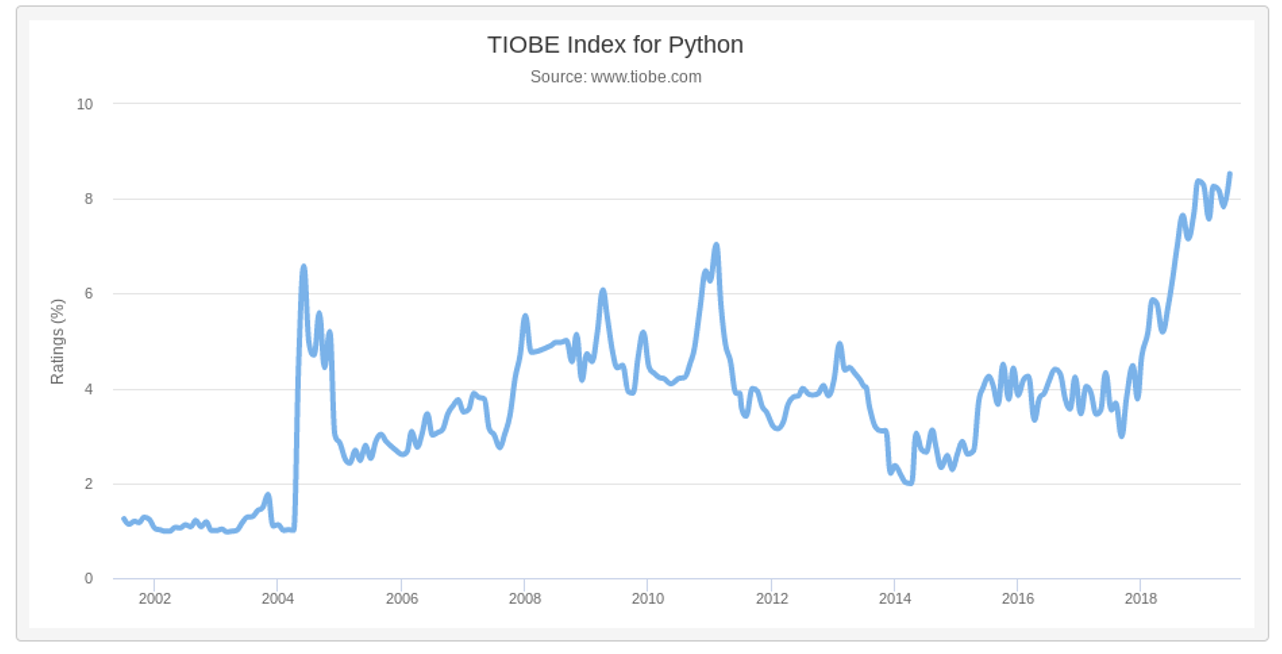
\includegraphics[width=\textwidth]{tiobe}
\centering
\end{figure}



หากเปรียบเทียบกับภาษาโปรแกรมมิ่งอื่น ๆ แล้ว Python มีไวยากรณ์ภาษา (Syntax) ที่สามารถอ่านง่าย เข้าใจได้ง่าย และเรียนรู้ง่าย Python จึงเป็นภาษาที่เหมาะสมสำหรับการสอนการเขียนโปรแกรมโดยเฉพาะอย่างยิ่งในระดับเบื้องต้น อีกทั้งยังเป็นภาษาที่ยืดหยุ่นสามารถพัฒนาได้บน ระบบปฏิบัติการที่หลากหลาย อาทิ  Windows, Linux, OS/2, MacOS, iOS และ Android นอกจากนี้ โปรแกรมเมอร์ทั่วโลกได้พัฒนาไลบรารี (Libraries) ขึ้นมาจำนวนมากสำหรับต่อยอด การทำงานของภาษา Python พื้นฐาน เช่น Django, Numpy, Pandas, Matplotlib, Flask, Web2py เป็นต้น \cite{Pyt19}

\section{Python ทำงานอย่างไร}

ภาษาโปรแกรมมิ่งระดับสูงจะต้องถูกโปรแกรมแปลภาษา เช่น คอมไพเลอร์ (Compiler) หรือ อินเทอร์พรีเตอร์ (Interpreter) ทำการแปลภาษาระดับสูงให้กลายเป็นภาษาเครื่องที่คอมพิวเตอร์เข้าใจก่อน \cite{Mar13} ภาษาตระกูลที่ต้องใช้ Compiler เพื่อแปลงเป็นภาษาคอมพิวเตอร์ซึ่งเป็นภาษาที่มนุษย์อ่านไม่ออกแล้วจึงจะทำงานได้ เช่น ภาษา Java ภาษา C หรือภาษา C++ ภาษาพวกนี้จะได้โปรแกรมที่ทำงานรวดเร็วมาก แต่ก็ยากที่จะเรียนรู้ในช่วงการฝึกฝนการเขียน Programming ใหม่ๆ \cite{Pau16}

แต่สำหรับภาษา Python เมื่อได้ Source code ที่เป็นนามสกุลไฟล์ \texttt{.py} แล้ว โปรแกรมจะถูกคอมไพล์โดยคอมไพเลอร์ของ Python เพื่อแปลคำสั่ง Python ให้เป็นคำสั่งแบบ Bytecode และบันทึกไว้ในไฟล์นามสกุล \texttt{.pyc} ต่อมาเมื่อผู้ใช้ต้องการ Run ไฟล์นี้ อินเทอร์พรีเตอร์ (Interpreter) ก็จะแปลง Bytecode เป็นภาษาเครื่องสำหรับการดำเนินการโดยตรงบนฮาร์ดแวร์ \cite{Bea13} อาจเรียกได้ว่า Python เป็นภาษาลูกครึ่งและเรียนรู้ได้ง่าย เหตุผลที่ Python ทำการคอมไพล์เป็น Bytecode เป็นรหัสกลางไว้ก่อนนั้น นั่นก็เพราะ Python ถูกออกแบบมาให้เป็นภาษาการเขียนโปรแกรมที่ไม่ขึ้นกับแพลตฟอร์ม ซึ่งหมายความว่ามีการเขียนโปรแกรมหนึ่งครั้ง แต่สามารถเรียกใช้งานบนอุปกรณ์ใดก็ได้ แต่จะต้องติดตั้ง Python เวอร์ชันที่เหมาะสม 

\section{อัลกอริทึม (Algorithm) และ ผังงาน (Flowchart)}

อัลกอริทึม (Algorithm) หมายถึง กระบวนการทีละขั้นตอนเพื่อแก้ไขปัญหาที่กำหนดอย่างชัดเจน โดยทั่วไปจะมีสามขั้นตอนหลัก คือ มีการนำเข้าข้อมูลหรืออินพุต แล้วนำมาประมวลผล และแสดงผลลัพธ์ออกมา \cite{Ari19} ตัวอย่างเช่น โจทย์ให้หาค่าเฉลี่ยของตัวเลขที่รับมาจากผู้ใช้จำนวนสามค่า จะสามารถเขียนเป็นขั้นตอนได้ดังนี้คือ

ขั้นตอนที่หนึ่ง การนำเข้าข้อมูล
\begin{enumerate}[noitemsep]
\item แจ้งให้ผู้ใช้ป้อนหมายเลขที่หนึ่ง
\item แจ้งให้ผู้ใช้ป้อนหมายเลขที่สอง
\item แจ้งให้ผู้ใช้ป้อนหมายเลขที่สาม
ขั้นตอนที่สอง การประมวลผลข้อมูล
\item คำนวณผลรวมของเลขทั้งสามจำนวน
\item หารผลรวมด้วยสาม
ขั้นตอนที่สาม การแสดงผลลัพธ์
\item แสดงผลลัพธ์ออกทางหน้าจอ
\end{enumerate}

ส่วนผังงาน (Flowchart) เป็นการนำเสนอการไหลของอัลกอริทึมในรูปแบบของสัญลักษณ์จากคำสั่งหนึ่งไปยังอีกต่อไปจนถึงจุดสิ้นสุดของอัลกอริทึม \cite{Cor09} สัญลักษณ์ที่ใช้บ่อยสำหรับผังงานมีดังต่อไปนี้


\begin{figure}[h]
\caption{สัญลักษณ์ผังงาน (Flowchart)}
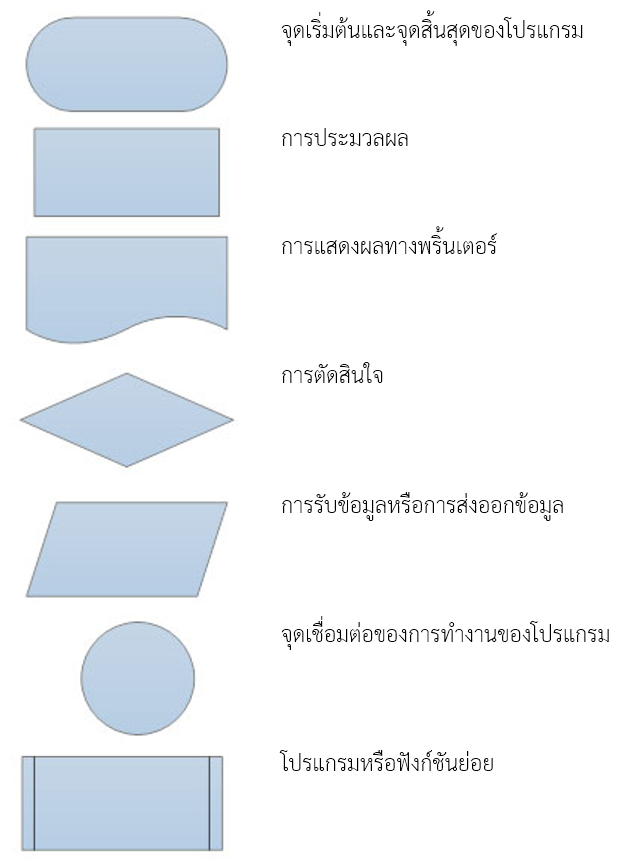
\includegraphics[width=10cm]{flowchart}
\centering
\end{figure}

ตัวอย่างการเขียนผังงานจากอัลกอริทึมด้านบนสามารถเขียนได้ดังนี้


\begin{figure}[h]
\caption{ตัวอย่างการเขียนผังงาน}
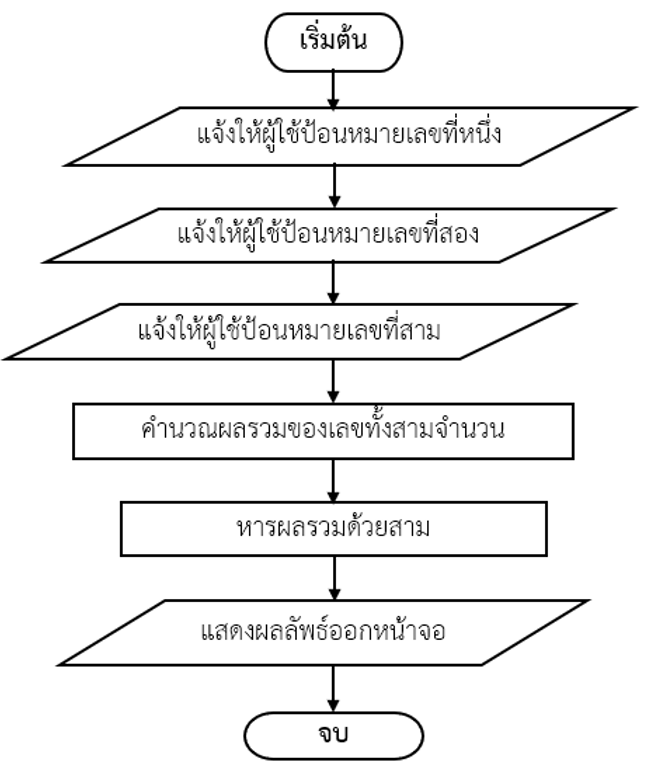
\includegraphics[width=10cm]{flowchartexample}
\centering
\end{figure}

\section{การติดตั้งโปรแกรม Python Runtime}

การติดตั้งโปรแกรม Python Runtime คือการติดตั้งโปรแกรมที่ทำให้นักพัฒนาซอฟต์แวร์สามารถใช้งานโปรแกรมที่เขียนขึ้นด้วยภาษา Python เองได้ ให้เข้าที่เว็บไซต์ \url{https://www.python.org/} \cite{Pyt19} ไปที่ Download for Windows แล้วเลือก Python 3.7.0 แล้วทำการติดตั้งให้เรียบร้อยลงในเครื่อง และให้เลือก Add Python 3.7 To Path เพื่อที่จะสามารถใช้ Python ได้ที่ Command Line หลังจากนั้นจะเห็นได้ว่าที่สตาร์ทเมนูโปรแกรม Python 3.7 จะถูกสร้างขึ้น ในโฟลเดอร์นี้จะมีโปรแกรมชื่อว่า Idle ซึ่งเป็น Integrated Development Environment หรือ เครื่องมือที่ช่วยในการพัฒนาโปรแกรมที่ใช้งานง่ายๆ เหมาะแก่การเขียนโปรแกรมเบื้องต้น โดยจะมีทั้ง Text Editor และ Interactive Shell เวลาใช้งานควรเปิดไว้ 2 หน้าต่าง ด้านซ้ายมือเป็น Source code ด้านขวามือเป็น Python Shell เพื่อใช้ดูผลลัพธ์ในการ Run โปรแกรมที่เขียนขึ้น

\begin{figure}[h]
\caption{การ Download Python 3.7}
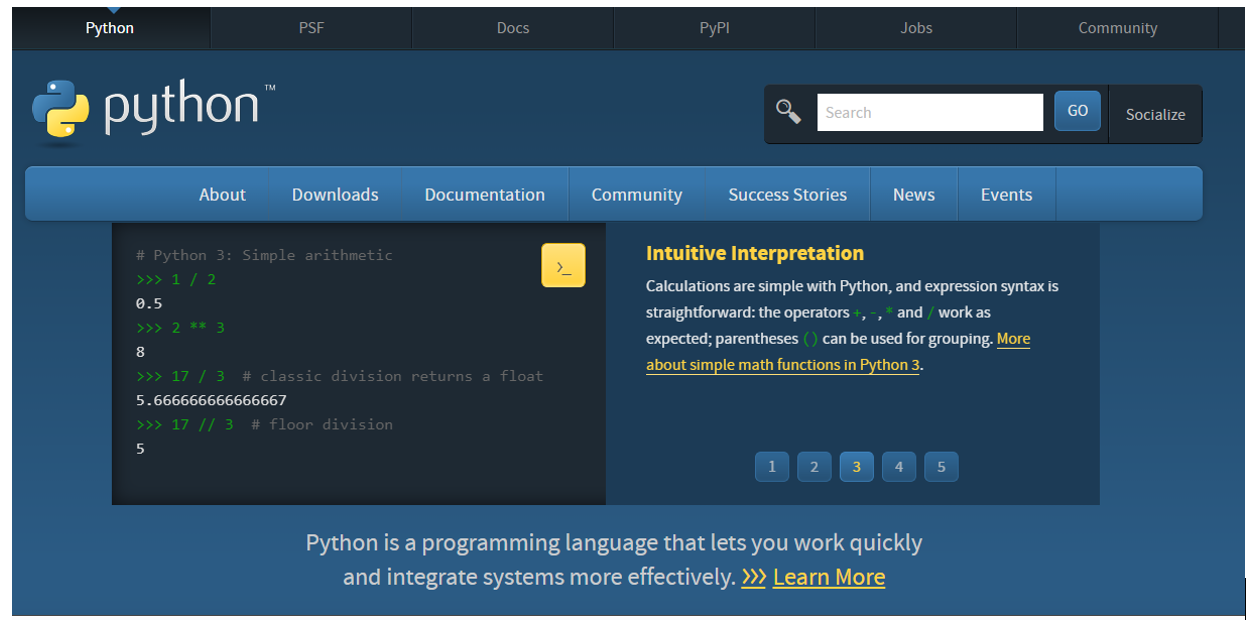
\includegraphics[width=\textwidth]{downloadpython}
\centering

\end{figure}

\begin{figure}[h]
\caption{เลือก Add Python 3.7 to PATH}
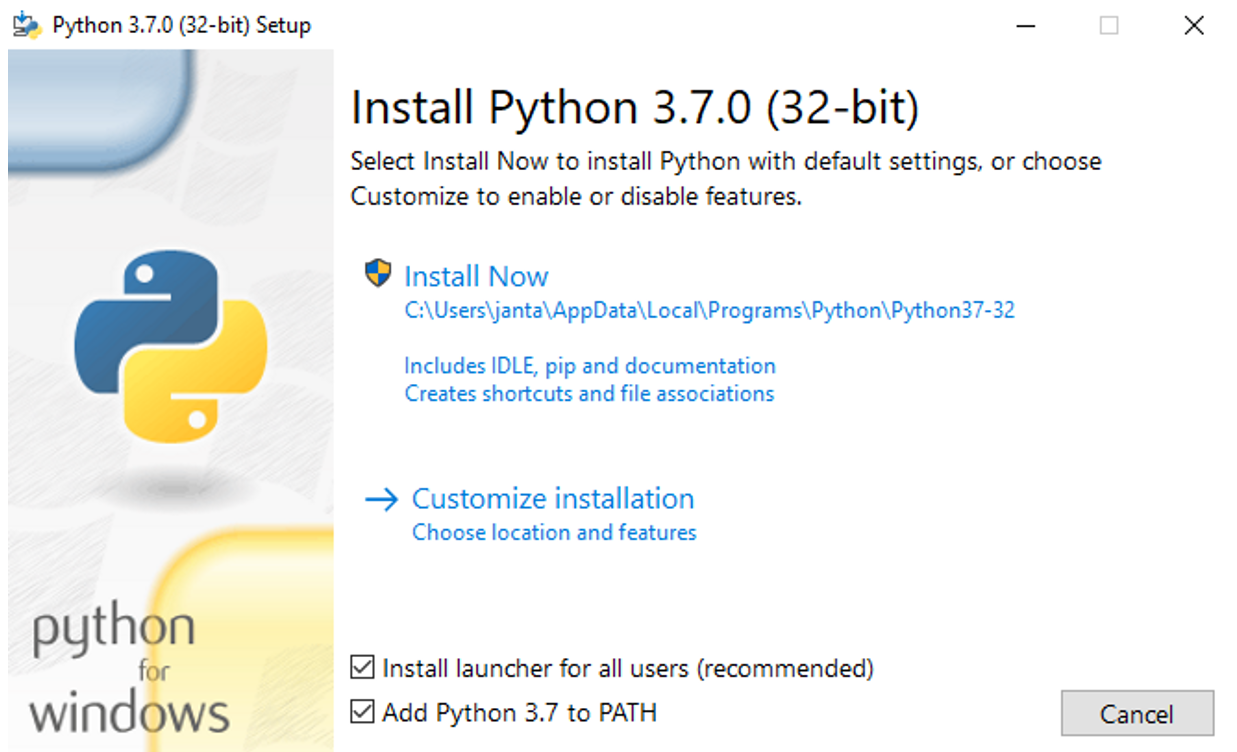
\includegraphics[width=\textwidth]{installpython}
\centering

\end{figure}


\begin{figure}[h]
\caption{โฟลเดอร์ Python 3.7 }
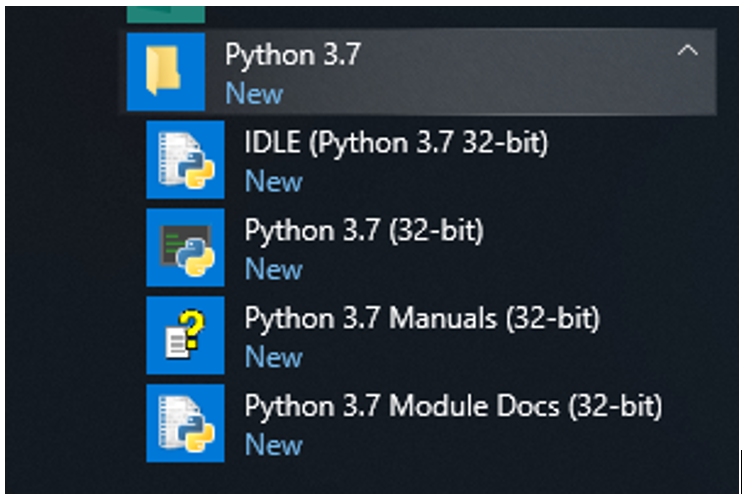
\includegraphics[width=10cm]{idle}
\centering

\end{figure}


\begin{figure}[h]
\caption{ตัวอย่างหน้าโปรแกรม Idle หน้า Editor}
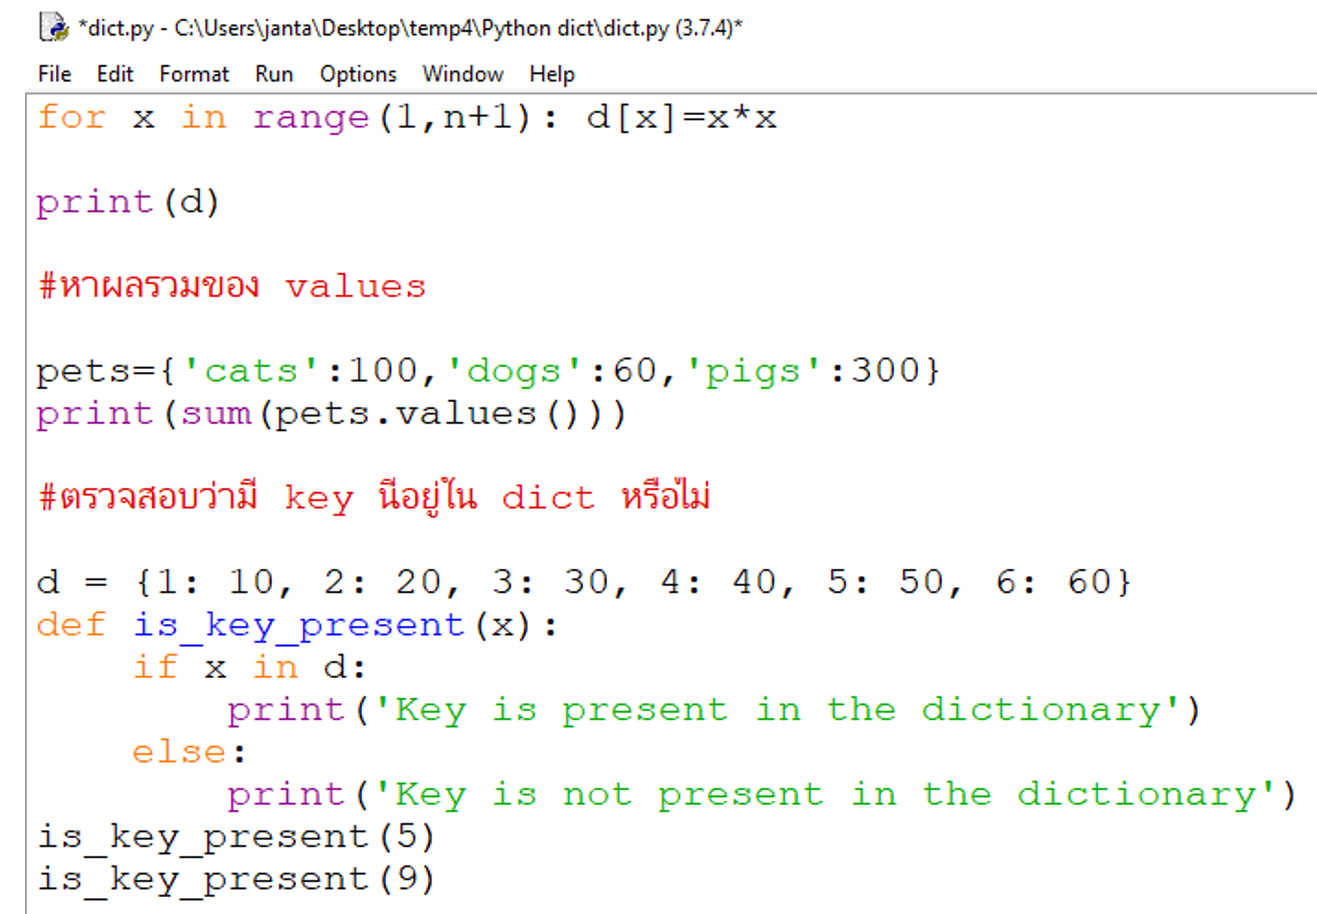
\includegraphics[width=\textwidth]{idlescreen}
\centering

\end{figure}

\begin{figure}[h]
\caption{ตัวอย่างหน้าโปรแกรม Idle หน้า Python Shell}
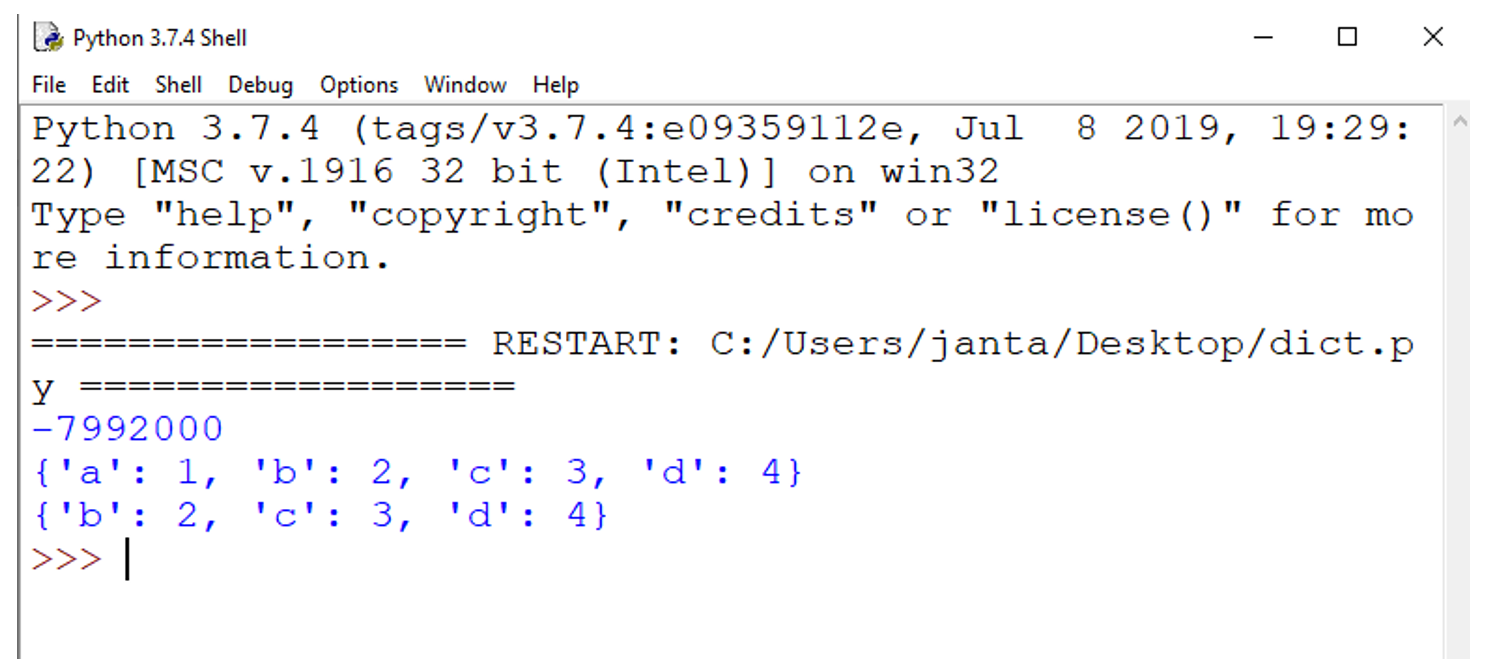
\includegraphics[width=\textwidth]{shell}
\centering

\end{figure}






